\documentclass{article}

\usepackage{times}
\usepackage{graphicx}
\usepackage{subfigure}
\usepackage{mdwlist}
\usepackage{bbm}

\usepackage{natbib}

\usepackage{algorithm}
\usepackage{algorithmic}

\usepackage{hyperref}

\newcommand{\theHalgorithm}{\arabic{algorithm}}

%\usepackage{icml2014} 
\usepackage[accepted]{icml2014}

\usepackage{amsmath}
\DeclareMathOperator*{\argmin}{arg\,min}


\icmltitlerunning{Streaming Entity-Based Document Filtering using Distributed Non-Parametric Representations}

\begin{document} 

\twocolumn[
\icmltitle{Streaming Entity-Based Document Filtering \\ using Distributed Non-Parametric Representations}

\icmlauthor{Ignacio Cano}{icano@cs.washington.edu}
\icmladdress{University of Washington, P. Allen Center, 185 Stevens Way, Seattle, WA 98195 USA}
\icmlauthor{Sameer Singh}{sameer@cs.washington.edu}
\icmladdress{University of Washington, P. Allen Center, 185 Stevens Way, Seattle, WA 98195 USA}
\icmlauthor{Carlos Guestrin}{guestrin@cs.washington.edu}
\icmladdress{University of Washington, P. Allen Center, 185 Stevens Way, Seattle, WA 98195 USA}

\icmlkeywords{non-parametric clustering, nlp, word embeddings, vital filtering, streaming}

\vskip 0.3in
]

\begin{abstract} 

Most studies that deal with large corpora of text documents have focused on identifying references to target entities as well as studying their topics evolution over time. However, current systems are unable to handle streaming data, they do not partition entities' references according to topics nor identify the references' vitalness.
In this paper we introduce a distributed, non-parametric representation of documents that addresses the above limitations. We propose a distributed word embedding representation of entities' contexts. Each context is described by topic clusters that are estimated in a non-parametric manner. Further, we associate a staleness measure to each entity and topic cluster, dynamically estimating their relevances based on document frequencies.
This approach of distributed word embeddings, non-parametric clustering, and staleness measure, provides an accurate representation of entities' contexts appropriate for streaming settings, while addressing the aforementioned constraints.


\end{abstract} 

\section{Introduction}
\label{intro}

\citet{frank12} observed a considerable time lag between the publication date of cited articles and the date of the corresponding citations created in Wikipedia. The median time is over a year, and the distribution has a long and heavy tail. This gap could be drastically reduced if automatic systems could suggest relevant documents to editors as soon as they are published.

However, when processing a large corpus of text documents, practitioners are often concerned in finding references to entities of interest \cite{RaoMD10, choi2007}, and studying their topics distributions over time \cite{blei12}. Current tools are somewhat limited; they do not handle online settings, and they do not cluster entities' references according to topics nor identify the references' importance.

Recent studies \cite{xitong13, bouvier13, efron13, zhang13, bellogin13} have centered their attention on solving the above problems with supervised methods, using mainly document, document-entity and temporal level features. \citet{Turian10wordrepresentations} showed that by using unlabeled examples to reduce data sparsity in the labeled training data, semi-supervised approaches can improve the generalization accuracy of those supervised systems.

We therefore introduce a semi-supervised approach suitable for streaming settings that uses a distributed word embedding and a non-parametric topic cluster representation of entities' contexts. We also include a staleness measure that approximates the relevance of each entity and its topic clusters according to document frequencies. Further, we update the topic identities, number of topics, and the entities and topics staleness in an online fashion, observing only a single document at a time.

This combination of distributed word embeddings, non-parametric clustering, and staleness measure provides an efficient yet accurate representation of entities' contexts that can be updated in a streaming manner, thus addressing the document filtering requirements on large streams of text.

We present experimental results demonstrating the benefits of our method and show that it surpasses previous supervised approaches in TRECKBA14 Vital Filtering task.

\section{Background}
\label{background}

\subsection{Problem Setup}
\label{setup}

We assume a set of $m$ target entities $E = \left\{ {e_1, ..., e_m}\right\}$. We further assume a set of $n$ documents $D = \left\{ {d_{1}, ..., d_{n}}\right\}$ that arrive in chronological order. 
 
Each document is a sequence of sentences composed by collections of words, annotated with NLP tools.
Further, we assume w.l.o.g. that every document in $D$ refers to a single entity $e \in E$. For illustrative purposes we let $e\mathord{=}Barack\hspace{1mm}Obama$.

We represent each $d_i \in D$ as a compound of a timestamp $t_i$ and a set of $p$ words $W_i = \left\{ {w_{i1}, ..., w_{ip}}\right\}$ located around (and including) mentions to the entity $e$. A mention to $e$ is found by a string matching algorithm that searches for exact matches of canonical and surface form names of the entity $e$.

We assume an online setting, i.e. the algorithm should provide predictions for documents arriving at time $t$ before seeing documents arriving at time $t+1$.

Further, documents can be categorized as follows:

\begin{itemize*}
    \item $Vital$: the document contains information that at the time it enters the stream, it drives an update to the entity $e$ with timely, new information about the entity's current state, actions or situation, e.g. ``Barack Obama has been elected President''.
    \item $Non\mathord{-}Vital$: the document contains information that can be used when building an initial profile of the entity $e$, it means that the document is possibly citable but the information is not timely, e.g. ``Barack Obama was born on August 4th, 1961''.
\end{itemize*}

\subsection{Word Embeddings}
\label{emb}

A word embedding is a dense, low-dimensional, and real-valued vector associated with a word. Each dimension of the embedding represents a latent feature of the word, and hopefully captures useful syntactic and semantic properties \cite{Turian10wordrepresentations}.

The learned vectors computed using neural networks are very attractive because they explicitly encode many linguistic regularities and patterns. Many of these patterns can be represented with simple algebraic operations. For example, the result of $v_{paris} - v_{france} + v_{germany}$ is closer to $v_{berlin}$ than to any other word vector \cite{mikolovChen,mikolovYih}.

Given the recent fast estimation of embedding representations at very large scale, there is rising interest in vector-space word embeddings and their use in NLP \cite{Arvind14}.

\section{Method}
\label{approach}

Given a stream of documents $D$ that refer to entity $e$, the task at hand is to predict whether those documents are $vital$ or $non\mathord{-}vital$ to $e$. For this, we propose a three-step method: 1) represent documents with embeddings computed from sets of words in each document, 2) represent the entity's context using non-parametric topic clusters, and 3) estimate the novelty of the document information with respect to entity $e$ using a staleness measure.

In section \ref{docwordemb} we describe the way to determine the word embedding representation of a document given the set of words located close to mentions of entity $e$. In section \ref{non}, we introduce the non-parametric representation of the entity's context. Finally, in section \ref{staleness} we present the staleness measure, which is a good indicator of the novelty of the information contained in a document with respect to $e$.

\subsection{Context Embedding Representation of Documents}
\label{docwordemb}

Topic models are a class of statistical models for collections of documents that represent documents as admixtures over topics. More specifically, each topic is modeled as a distribution over words, and each document is a mixture of such topics \cite{InouyeRD14}. Though they can be easily extended and embedded in other models, they do not generalize to new, unseen documents and they are prone to overfitting. 

In order to address the lexical sparsity and generalize to unseen documents, given the nice properties exposed in section \ref{emb}, we propose to represent entity's contexts in documents by their mean word embedding vector.

We define a function $f : w \rightarrow v_w \in \mathbf{R^d}$ that computes the word embedding representation of the word string $w$. We further define a function $g : W \rightarrow v_W \in \mathbf{R^d}$ that computes the mean word embedding representation of the set of words in $W$ as defined in Equation \ref{wordembedding}.

\begin{equation}
\label{wordembedding}
g(W) = v_W = \frac{1}{|W|} \sum_{w \in W}{f(w)}
\end{equation}

Given the document $d_i \in D$ that refers to entity $e$ and contains the words $w_i \in W_i$, we can compute its vector representation using function $g$ as follows:

\begin{equation}
\label{wordembedding1}
v_{d_i} = v_{W_i} = g(W_i)
\end{equation}

With this, we intend to capture the context where the entity $e$ is mentioned in a document, i.e. the topic, and represent it with a dense, low-dimensional vector.

Further, let's denote $W_{i_n}$ to the set of all nouns in $W_i$, where $W_{i_n} \subseteq W_i$, and $W_{i_v}$ to the set of all verbs in $W_i$, where $W_{i_v} \subseteq W_i$. We can simply compute the mean embedding vector of all the nouns and verbs that appear in the context of entity $e$ using function $g$, as shown below:

\begin{equation*}
\label{nouns}
v_{d_{i_n}} = v_{W_{i_n}} = g(W_{i_n})
\end{equation*}

\begin{equation*}
\label{verbs}
v_{d_{i_v}} = v_{W_{i_v}} = g(W_{i_v})
\end{equation*}

Being able to compute individual embeddings for different word types is a flexibility our method provides that might better encapsulate the truth underlying context (topic) of the document.

\subsection{Non-parametric Clustering}
\label{non}

The context of entity $e$ is further represented by topic clusters, which are estimated in a non-parametric manner by assuming that the entity's context in a single document belongs to a single topic. As we are dealing with a streaming setting, topic clusters do evolve over time, i.e. members of each cluster change over time. We therefore represent each topic cluster by the mean embedding vector of the documents in that cluster at a certain timestamp.

Mathematically, the vector representation of the $j$-th topic cluster at timestamp $t_i$, $c^j_i$, can be computed using Equation \ref{nonparamclust}.

\begin{equation}
\label{nonparamclust}
v_{c^j_i} = \frac{1}{|D^j_i|} \sum_{d \in D^j_i}{v_d}
\end{equation}
where $D^j_i$ is the subset of all the documents that belong to cluster $j$ at timestamp $t_i$, and $\forall\hspace{1mm}d_q \in D^j_i, t_q \leq t_i$.

The number of topic clusters for the context of entity $e$ is unknown beforehand. Initially, the entity's context does not have topic clusters. We create the first topic cluster for the entity's context on its first occurrence in the training data. After creating the first cluster for the context, a new topic cluster is created when the cosine distance between the word embedding representation of the new arriving document with every topic cluster center of the entity is greater than or equal to $\alpha$, where $\alpha$ is an hyperparameter of the model, and $0 \leq \alpha \leq 1$. Our approach is closely related to the online non-parametric clustering procedure described in \citet{Arvind14}.

In case the distance is less than $\alpha$, we add the incoming document to the closest topic cluster and update its center. 

More formally, $\forall\hspace{1mm}c^j_{i-1}$, at time $i$, document $d_i$ is added to the topic cluster that solves the following optimization problem:\\

\centerline{$\underset{j}{\argmin}$\;\; $dist(v_{d_i}, v_{c^j_{i-1}})$} 
\medskip
\centerline{\text{subject to} $dist(v_{d_i}, v_{c^j_{i-1}}) < \alpha$}

where $dist(\cdot,\cdot)$ is the cosine distance defined in Equation \ref{cosine}

\begin{equation}
\label{cosine}
dist(x,y) = 1 - \cos(x,y) = 1 - \frac{x \cdot y}{||x||||y||}
\end{equation}

The $j$-th topic cluster at time $i$ is updated, and therefore composed by the subset of documents $D^j_i \subseteq D$, where $D^j_i = D^j_{i-1} \cup \left\{ {d_i}\right\}$.

%\begin{algorithm}[tb]
%   \caption{Non-parametric Clustering}
%   \label{nonparamclustering}
%\begin{algorithmic}
%   \STATE {\bfseries Input:} $doc=doc\_word\_embedding(d, e, c)$, and topic clusters list $tcs$ for entity $e$
%   \STATE {\bfseries Output:} new or updated topic cluster $tc$
%   \STATE {\bfseries Body:}
%   \STATE Initialize $tc = nil$
%   \IF{$tcs$ {\bfseries is empty}}
%    \STATE $tc = create\_topic\_cluster(center\mathord{=}doc)$
%    \STATE $tcs.append(tc)$
%   \ELSE
%     \STATE $dist, i \mathord{=} \min_{\forall{i \in tcs}}{cosine\_dist(tcs[i].center, doc)}$
%     \IF{$dist >= \alpha$ }
%        \STATE $tc = create\_topic\_cluster(center\mathord{=}doc)$
%        \STATE $tcs.append(tc)$
%     \ELSE
%        \STATE $tc = update\_topic\_cluster(tcs[i], doc)$
%     \ENDIF
%   \ENDIF
%   \STATE return $tc$
%\end{algorithmic}
%\end{algorithm}

As an example, let's assume document $d_1$ appears in the stream, and talks about the days Barack Obama was a Senator. As is the first document referring to the entity Obama, we add $d_1$ to a new topic cluster $senator$. Then, document $d_2$ appears in the stream. It refers to Obama as being elected President of the United States. The distance with the previous cluster $senator$ is greater than $\alpha$, therefore the algorithm proceeds to add $d_2$ to a new topic cluster $president$. Finally, $d_3$ enters the stream. It talks about Obama as the current President of the U.S. The algorithm compares its distance to the previous clusters and finds that is closest to the $president$ cluster. The distance is less than $\alpha$, hence it adds $d_3$ to the $president$ cluster and updates the cluster center.

\subsection{Staleness}
\label{staleness}

As mentioned in section \ref{setup}, the notion of $vitalness$ is closely related to the timeliness of the new information. We include a staleness feature $\lambda_i$, which is dynamically updated over time, and $0 < \lambda_i \leq 1$. Low staleness aims to represent vital documents.

This staleness measure can be used both for entities and topic clusters.

The staleness update is a two-step process, an exponential decrease followed by a constant increase.
We denote the staleness decrease as $\lambda^{dec}_i$, and is controlled by the hyperparameter $\gamma_d$ following an exponential decay model.
\begin{equation}
\label{decrease}
\lambda^{dec}_i = \lambda^{inc}_{{i-1}} \exp{(-\gamma_d \frac{t_i-t_{i-1}}{T})}
\end{equation}
where $\gamma_d \geq 0$, $t_i$ is the $i$-th document timestamp, $t_{i-1}$ is the $i-1$ document timestamp, $T$ is a normalizing constant, and $\lambda^{inc}_{i-1}$ is the staleness increase (defined below) at a previous timestamp.
In case we use staleness as an entity's measure, $\lambda^{inc}_{i-1}$ alludes to the staleness of the previous document in the stream that refers to the same entity as document $i$.
If we use staleness as a topic cluster's measure, $\lambda^{inc}_{i-1}$ refers to the staleness of the previous document that belongs to the same topic cluster as document $i$.

On the other hand, the staleness increase is denoted as $\lambda^{inc}_i$, and is regulated by $\gamma_i$ according to the following expression
\begin{equation}
\lambda^{inc}_i = 1 - (1 - \lambda^{dec}_i) \gamma_i
\end{equation}
where $0 \leq \gamma_i \leq 1$.

The final staleness feature reported for the $i$-th document is $\lambda^{dec}_i$.

\subsubsection{Examples}

Figures \ref{stalenesslow} and \ref{stalenessmedium} illustrate some toy examples to further understand the intuition behind staleness.

Figure \ref{stalenesslow} intends to show an example of an entity with a decreasing staleness. There are almost no documents in the stream referred to that entity. As soon as some activity is detected, i.e. a document mentioning the entity appears ($t\mathord{=}10$), a slight increase in the curve is seen. Given the fact that there's no much information about the entity, every new document would drive an update to the entity's profile, strongly suggesting vitalness.

\begin{figure}[h!]
\centering
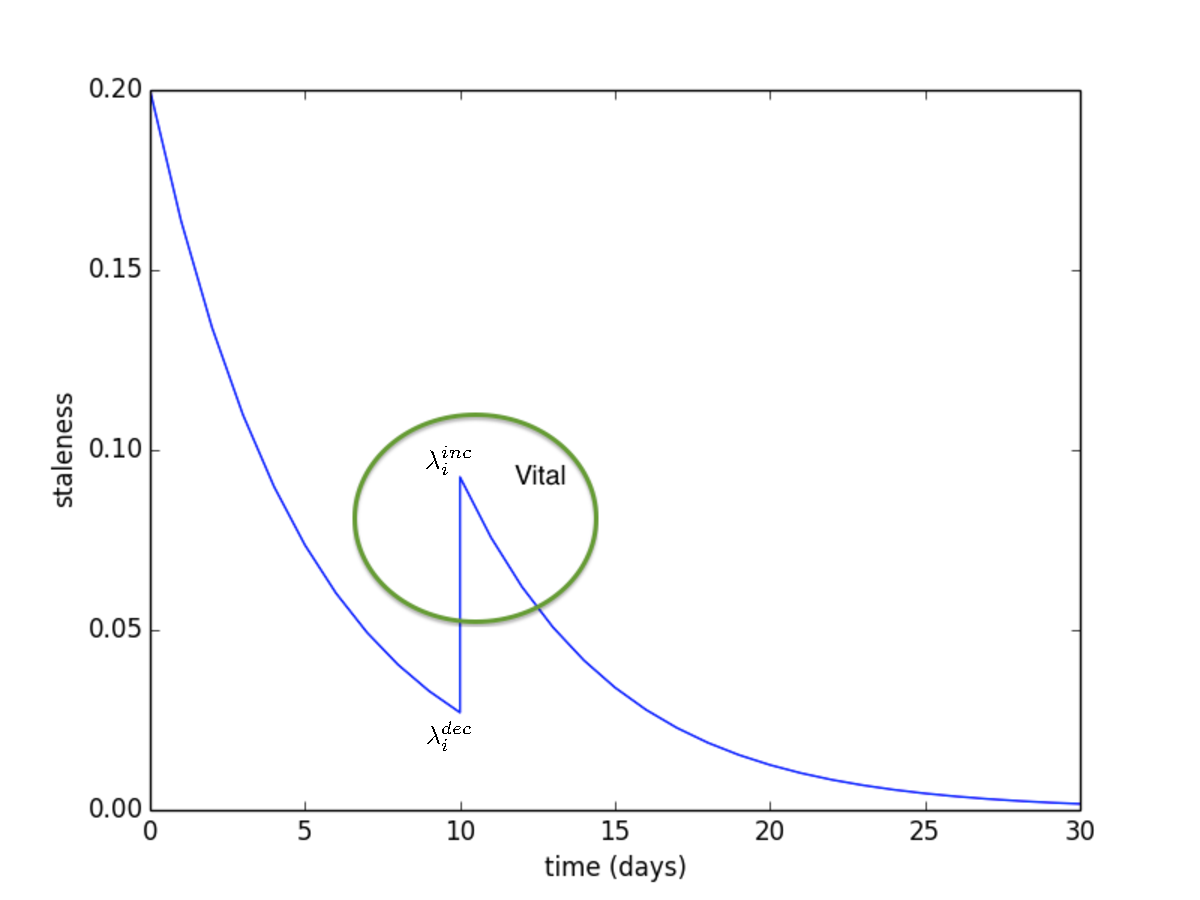
\includegraphics[width=.5\textwidth]{staleness1.pdf}
\caption{Staleness of Unpopular Entity}
\label{stalenesslow}
\end{figure}

Figure \ref{stalenessmedium} aims to represent staleness of an entity with fluctuating activity levels in the stream of documents. At time $t\mathord{=}10$, a main event involving the entity starts and continues for a long period of time, showing a growing trend in popularity. 
At the beginning, those documents can be considered vital, but as time goes by and documents continue commenting on the same event, the information starts staling, clearly indicating non-vitalness.
Near $t\mathord{=}40$, the event can be considered over, a steep decrease in popularity is shown. At a later time, $t=50$, a new event occurs, which denotes vitalness.

\begin{figure}[h!]
\centering
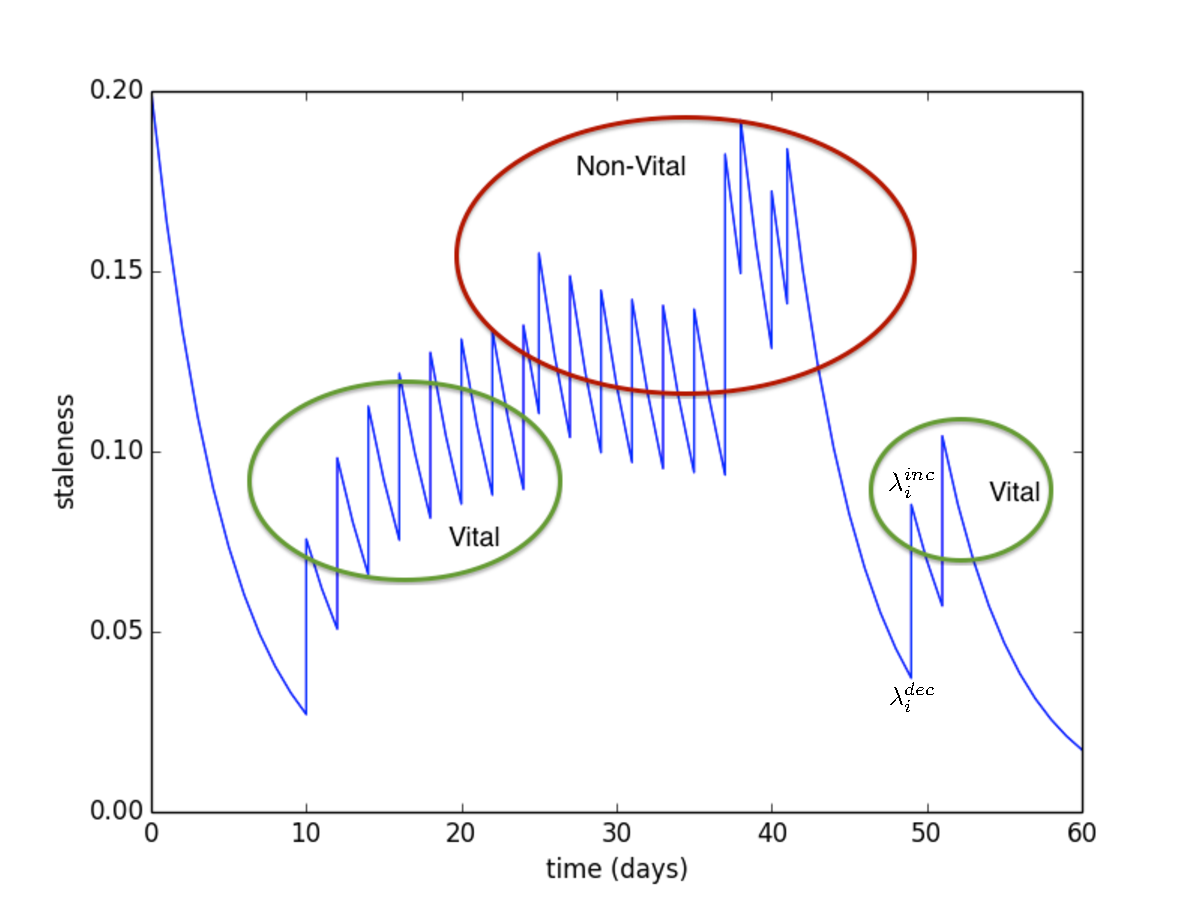
\includegraphics[width=.5\textwidth]{staleness2.pdf}
\caption{Staleness of Entity with Fluctuating Popularity}
\label{stalenessmedium}
\end{figure}


\section{Evaluation}
\label{evaluation}

\subsection{Data}
\label{data}

To assess our method we use TRECKBA14 stream corpus. It has around 20M documents annotated with BBN's Serif NLP tools, including within-doc coref and dependency parse trees. Further, we use the 71 target entities given by TRECKBA14 organizers for the Vital Filtering task. Among the 20M documents, around 28K have truth labels. From these, only 8K are training instances while the rest are test examples.

\subsubsection{Preprocess}

We preprocess the corpus to filter the documents that contain exact string matches to the target entities names, including canonical and surface form names.

\subsubsection{Categories}
\label{subcat}

TRECKBA14 corpus contain documents that do not refer to the target entities, even though they may contain references to them. We therefore need to introduce a new category of documents, $non\mathord{-}referent$. 

A $non\mathord{-}referent$ document means that it doesn't refer to a target entity or the context is so ambiguous that is impossible to decide whether the mention refers to an entity or not. An example for the former case is ``Barack Ferrazzano provides a wide range of business-oriented legal''. For the latter, an example is ``Barack is a great father and a better husband''. The mention ``Barack'' may refer to any married parent named Barack, therefore, we consider it $non\mathord{-}referent$.

The $vital$ and $non\mathord{-}vital$ classes described in section \ref{setup} fall into a $referent$ category, which contains documents that refer to the target entities.

\subsection{Features}
\label{feat}

A summary of the features we use is presented below. Basic features are borrowed from \cite{jingang13}.

\begin{itemize*}
  \item \textbf{Basic}
    \begin{itemize*}
      \item \textit{Document}
        \begin{itemize*}
            \item $log(len(d))$: log of the length of document $d$
            \item $source(d)$: discretized source of document $d$
        \end{itemize*}
      \item \textit{Document-Entity}
        \begin{itemize*}
            \item $n(d,e)$: \# of occurrences of target entity $e$ in document $d$
            \item $n(d,e^p)$: \# of occurrences of partial name of target entity $e$ in document $d$
            \item $fpos(d,e)$: position of first occurrence of entity $e$ in document $d$
            \item $fpos_n(d,e)$: $fpos(d,e)$ normalized by document length
            \item $fpos(d,e^p)$: position of first occurrence of partial name of entity $e$ in document $d$
            \item $fpos_n(d,e^p)$: $fpos(d,e_p)$ normalized by document length
            \item $lpos(d,e)$: position of last occurrence of entity $e$ in document $d$
            \item $lpos_n(d,e)$: $lpos(d,e)$ normalized by document length
            \item $lpos(d,e^p)$: position of last occurrence of partial name of entity $e$ in document $d$
            \item $lpos_n(d,e^p)$: $lpos(d,e^p)$ normalized by document length
            \item $spread(d,e)$: $lpos(d,e) - fpos(d,e)$
            \item $spread_n(d,e)$: $spread(d,e)$ normalized by document length
            \item $spread(d,e^p)$: $lpos(d,e^p)\mathord{-}fpos(d,e^p)$
            \item $spread_n(d,e^p)$: $spread(d,e^p)$ normalized by document length
        \end{itemize*}
    \end{itemize*}
  \item \textbf{Embeddings}
    \begin{itemize*}
        \item $mean(d)$: mean word embedding representation of document $d$
    \end{itemize*}
  \item \textbf{Non-parametric Clustering}
    \begin{itemize*}
        \item $min(mean(d),e)$: minimum distance of the mean word embedding representation of document $d$ to existent topic clusters of target entity $e$
        \item $avg(mean(d),e)$: avg distance of the mean word embedding representation of document $d$ to existent topic clusters of target entity $e$
        \item $zero(mean(d))$: $\mathbbm{1}_{0}{(d)}$, i.e. flag set to 1 if the mean word embedding representation of document $d$ is $0$
    \end{itemize*}
  \item \textbf{Staleness}
    \begin{itemize*}
        \item $stale(e)$: staleness of entity $e$
        \item $stale(e,c)$: staleness of topic cluster $c$ of target entity $e$
    \end{itemize*}
\end{itemize*}


\subsection{Experiments}
\label{expe}

Due to the fact that not all documents in the corpus refer to the target entities (section \ref{subcat}), we include an extra step in our classification process. We introduce an additional classifier, called $rnr$, which acts offline and classifies documents as $referent$ or $non\mathord{-}referent$.

Consequently, in every experiment, each document goes first through the $rnr$ classifier. Only the $referent$ documents outputted by $rnr$ are used as inputs to the $uv$ model, which discriminates between $vital$ and $non\mathord{-}vital$ documents, the overall focus of this work.

We use therefore two extremely randomized tree ensembles classifiers \cite{GEW06a} in cascade, each composed of 100 weak learners. Each tree in the ensembles has depth 150.

All the experiments use the same $rnr$ model trained with the basic features listed in section \ref{feat}. 
The different models differ on the features used to train and test the $uv$ classifier.

\begin{itemize*}
  \item {\textit{Baseline Single}}: baseline method that uses basic document and document-entity features. \citet{jingang13, bellogin13} have a similar method, though they train their models with more features.
  \item {\textit{Baseline Multi-task}}: another baseline method. It's similar to {\textit{Basic Single}} but it includes multi-task learning \cite{Caruana93multitasklearning}.
  \item {\textit{Embedding Combined}}: similar to {\textit{Basic Multi-task}}. It also includes the embeddings features. The word embeddings are computed using the pre-trained Google News dataset. Each document has a single combined embedding, which is calculated from the nouns, proper nouns and verbs found near the mentions to entities as explained in section \ref{docwordemb}.
  \item {\textit{Embedding POS}}: similar to {\textit{Embedding Combined}} but instead of a single combined embedding per document, it has one embedding per word type in each document, i.e. it computes separate embeddings for nouns, proper nouns and verbs. It uses the part of speech annotations in the documents to easily extract the different word types.
  \item {\textit{Mean Static}}: similar to {\textit{Embedding POS}}. It also includes the staleness measure, which is constant throughout the stream, as $\gamma_d = 0$ and $\gamma_i = 1$. No topic clusters are formed, this means that $\alpha = 1$.
  \item {\textit{Mean Dynamic}}: similar to {\textit{Embedding POS}}. Further, it includes the staleness measure, which fluctuates over time as $\gamma_d \neq 0$ and $\gamma_i \neq 1$. Still no topic clusters are formed, i.e. $\alpha = 1$.
  \item {\textit{Clustering Static}}: similar to {\textit{Mean Static}} in the sense that the staleness is constant over time, i.e. $\gamma_d = 0$ and $\gamma_i = 1$, but it also includes topic clusters by making $\alpha \neq 1$.
  \item {\textit{Clustering Dynamic}}: similar to {\textit{Mean Dynamic}} in the sense that the staleness fluctuates over time, i.e. $\gamma_d \neq 0$ and $\gamma_i \neq 1$, but it also adds topic clusters by making $\alpha \neq 1$.
\end{itemize*}

\section{Results \& Discussion}

Table \ref{res} shows the micro precision, recall and F1 results of the methods explained in \ref{expe}, computed using KBA official scorer tool. The \textit{Clustering} models use $\alpha=0.8$. Also, the \textit{Dynamic} methods use $\gamma_d=1$ and $\gamma_i=0.1$.

\begin{table}[H]
\center
\begin{tabular}{|c|c|c|c|c|} \hline
\textbf{Model} & \textbf{P} & \textbf{R} & \textbf{F1} \\ \hline\hline
{\textit{Baseline Single}} & 0.538 & 0.265 & 0.355 \\ \hline
{\textit{Baseline Multi-task}} & \textbf{0.607} & 0.414 & 0.492 \\ \hline
{\textit{Embedding Combined}} & 0.547 & \textbf{0.521} & \textbf{0.534} \\ \hline
{\textit{Embedding POS}} & 0.538 & 0.464 & 0.498 \\ \hline
{\textit{Mean Static}} & 0.573 & 0.476 & 0.520 \\ \hline
{\textit{Mean Dynamic}} & 0.572 & 0.482 & 0.524 \\ \hline
{\textit{Clustering Static}} & 0.569 & 0.490 & 0.527 \\ \hline
{\textit{Clustering Dynamic}} & 0.562 & 0.481 & 0.518 \\ \hline
\end{tabular}
\caption{TRECKBA14 Vital Filtering scores}
\label{res}
\end{table}

The {\textit{Embedding Combined}} approach has the overall best F1 on the $vital$ filtering task. Our two baselines ({\textit{Baseline Single}} and {\textit{Baseline Multi-task}}) perform as expected, i.e. have lower F1 than the other models. The F1 difference between the two baselines evidences that multi-task learning does work.

\begin{figure}[h!]
\centering
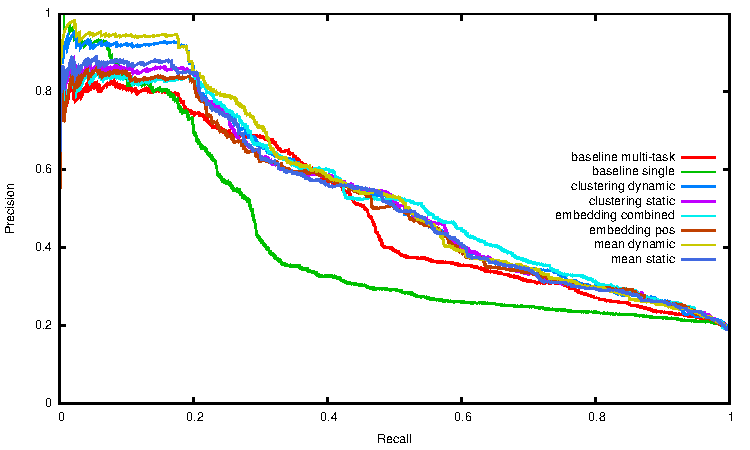
\includegraphics[width=.5\textwidth]{overlapped.pdf}
\caption{Precision-Recall}
\label{precrecall}
\end{figure}

The more advanced models perform better than both baselines. Using a combined embedding ({\textit{Embedding Combined}}) outperforms using individual embeddings representations for the different type of words ({\textit{Embedding POS}}).

Though the staleness and non-parametric clustering runs ({\textit{Mean Static}}, {\textit{Mean Dynamic}}, {\textit{Clustering Static}}, {\textit{Clustering Dynamic}}) perform slightly worse than the simple {\textit{Embedding Combined}} method, they illustrate the importance of these new features as they improve the performance of the {\textit{Embedding POS}} model.

Figure \ref{precrecall} further illustrates the precision-recall for the different methods listed in Table \ref{res}. It's worth noting that on low recall, the precision of the different models meets our expectations, the more complex methods, which include non-parametric clustering and staleness, outperform the simpler ones. Nevertheless, on high recall, {\textit{Embedding Combined}} takes the lead.

Table \ref{varyinggamma} shows the results for a variant of {\textit{Clustering Dynamic}}. As opposed to the {\textit{Clustering Dynamic}} in Table \ref{res}, this new version uses a single embedding representation instead of embeddings per word type. We show outputs using a low, medium and high $\gamma_i$, for $\alpha=0.6$. We further perform a scan on a long range of $\gamma_d$ to see its impact on the overall result. 

\begin{table}[H]
\center
\begin{tabular}{|c|c|c|c|c|} \hline
$\gamma_i$ & $\gamma_d$ & \textbf{P} & \textbf{R} & \textbf{F1} \\ \hline\hline
0.1 & 0.2 & 0.525 & \textbf{0.518} & 0.521 \\ \hline
0.1 & 0.5 & 0.537 & 0.514 & \textbf{0.525} \\ \hline
0.1 & 1   & 0.516 & 0.514 & 0.515 \\ \hline
0.1 & 20  & 0.512 & 0.506 & 0.509 \\ \hline
0.1 & 100 & \textbf{0.583} & 0.463 & 0.516 \\ \hline\hline
0.5 & 0.2 & \textbf{0.592*} & 0.479 & \textbf{0.530*} \\ \hline
0.5 & 0.5 & 0.537 & 0.523 & 0.529 \\ \hline
0.5 & 1   & 0.527 & 0.520 & 0.524 \\ \hline
0.5 & 20  & 0.516 & 0.504 & 0.510 \\ \hline
0.5 & 100 & 0.528 & \textbf{0.528} & 0.528 \\ \hline\hline
0.9 & 0.2 & 0.529 & 0.509 & 0.519 \\ \hline
0.9 & 0.5 & 0.533 & 0.520 & 0.526 \\ \hline
0.9 & 1   & 0.540 & 0.518 & \textbf{0.529} \\ \hline
0.9 & 20  & 0.521 & \textbf{0.529*} & 0.525 \\ \hline
0.9 & 100 & \textbf{0.586} & 0.460 & 0.516 \\ \hline
\end{tabular}
\footnotetext{Footnote}
\caption{Scores for variant of clustering dynamic with a single embedding and $\alpha=0.6$}
\label{varyinggamma}
\end{table}

We achieve the best result when $\gamma_i=0.5$ and $\gamma_d=0.2$, still lower than \textit{Embedding Combined} but better than previous {\textit{Clustering Dynamic}}. In general, lower $\gamma_d$ seems to be doing a better job. These results further reflect the importance of hyperparameter tuning.

Further, we present some qualitative results on topic clusters of the previous method. Table \ref{clusterresult} illustrates the top 5 words that appear more often in 4 random topic clusters computed for entity Lisa Brown.

\begin{table}[H]
\center
\begin{tabular}{|c|c|c|c|} \hline
\textbf{C1} & \textbf{C2} & \textbf{C3} & \textbf{C4} \\ \hline\hline
director & leader & counselor & vagina \\ \hline
executive & majority & doctors & state \\ \hline
white\_house & senate & welcomes & michigan \\ \hline
representative & state & usa & word \\ \hline
introduced & spokane & nutrition & floor \\ \hline
\end{tabular}
\caption{An illustration of 4 (out of 78) topic clusters extracted for entity Lisa Brown}
\label{clusterresult}
\end{table}

By doing some manual search on the entity Lisa Brown, we can confirm that the cluster elements make sense. Mrs. Brown is an American politician from the state of Michigan, who has been member of the Michigan State House of Representatives, and she is on the Executive Board of some association.
Even the word vagina is justifiable as she engaged in a heated debate about abortion legislation in Michigan.

Although Table \ref{varyinggamma} show some results for different $\gamma_i$ and $\gamma_d$, further experimental investigations are needed to account for the correct tunning of the hyperparameters of the model. Exploiting external resources such as Wikipedia entity pages to construct more features \cite{xitong12} should probably increase the overall accuracy of our method. It would also be interesting to assess the effects of using different pre-trained word embeddings.

\section{Related Work}
\label{related}

Streaming document filtering is related to several fields, including but not limited to, entity linking \cite{KBP11}, text categorization \cite{HLTCOE12}, news surveillance \cite{Steinberger14}.

Several comparative knowledge based population competitions have run in the recent past testifying on the great progress achieved in these fields \cite{gross_doucet_toivonen_trec12}. 

\citet{xitong12} presented one of the best performing systems in TRECKBA12. They created wider representations of entities' profiles based on a Wikipedia snapshot and considered the anchor text of all internal Wikipedia links as related entities. In TRECKBA13 competition, different families of methods were proposed, query expansion, classification, learning to rank. 

Our strategy is somewhat similar to \citet{jingang13} in the sense that we first target for a high recall system and then apply different classification methods to differentiate between $vital$ and $non\mathord{-}vital$ documents. Nevertheless, one key difference is that we do not exploit any external resources to construct features, e.g. we do not use Wikipedia entity pages nor existing citations in the Wikipedia page of an entity. 

Representing words as continuous vectors has been around for a while \cite{Hinton87, Elman90findingstructure}. The progress of machine learning techniques in recent years enabled training more complex models on much larger data sets \cite{mikolovChen}. One popular approach to increase accuracy in existing system is to use unsupervised methods to create word features, or to download word features that have already been produced \cite{Turian10wordrepresentations}. In our method, we do the latter, we use already induced word embedding features in order to improve its accuracy.

To our best knowledge, no recent techniques propose a combination of distributed word embeddings, non-parametric clustering and a staleness notion to solve this problem. 

The closest example we found that addresses the problem of staleness detection is \cite{gamon}, where he builds an association graph connecting sentences and sentence fragments, and uses some graph-based features as good indicators of lack of novelty.

\section{Conclusion \& Future Work}
\label{conclusion}

Filtering streaming documents to accelerate users filling knowledge gaps plays a crucial role in the maintenance and update of knowledge bases.
With the exponential increase of information on the web, it becomes critical to detect relevant documents and incorporate their information to entities in a timely manner \cite{jingang13}.

In this paper we introduce a semi-supervised learning model for document filtering tasks. We propose a distributed, non-parametric representation of documents suitable for streaming settings, that groups entities' references into topic clusters. Further, we present a notion of staleness computed per entity as well as per topic cluster, which dynamically estimates entities' and clusters' relevances.

Combining these three core ideas, distributed word embeddings, non-parametric clustering, and staleness, results in a more accurate representation of entities' contexts, and simultaneously addresses the filtering requirements of large corpora of streaming text documents.

Further work needs to be done. A possible line of future research would be exploring hierarchical clustering algorithms to better represent topic clusters. It would also be interesting to assess the effect of learning the hyperparameters of the model instead of just manual tuning them for the specific datasets.

\section*{Acknowledgments} 
 
This work was supported in part by the Argentine Ministry of Science, Technology and Productive Innovation and the TerraSwarm Research Center, supported by the STARnet phase of the Focus Center Research Program (FCRP). Any opinions, findings and conclusions or recommendations expressed in this material are those of the authors and do not necessarily reflect those of the sponsors.

\bibliography{summer_research_paper}
\bibliographystyle{icml2014}

\end{document} 


